\documentclass[a4paper,11pt]{article} 

% ===== Algunos paquetes a ser usados =====

% para poder escribir con tildes   
\usepackage[T1]{fontenc}           
\usepackage[utf8]{inputenc}        
\usepackage[spanish]{babel}        

\spanishdecimal{.}        
\usepackage{times}        

\usepackage{animate}        

% fuentes para escribir símbolos 
\usepackage{amsfonts}            
\usepackage{amssymb}             
\usepackage{amsthm}              
\usepackage{mathrsfs}            
\usepackage[centertags]{amsmath}    

% inclusión de graficos    
\usepackage{graphicx}      

% símbolo de grados    
\newcommand{\grad}{\hspace{-2.5mm}$\,\phantom{a}^{\circ}\,$}        

% ==================================== 

% ========= Referencias ==========           
\usepackage{hyperref}                        
% ================================           

% ========= Color ==========           
\usepackage[usenames,dvipsnames]{color}                         
% ================================           

% ===== Ajuste layout pagina =====           
\textheight=23cm                            
\textwidth=18cm                              
\topmargin=-1cm                              
\oddsidemargin=-1cm                           
\parindent=0mm                               
\usepackage{fancyhdr}                        
% ================================           

% ========= Comandos ==========           
\newcommand{\ds}{\displaystyle}         
\def\x{{\bf x}}                         
% ================================           

% ========= Tablas y otros ==========           
%\usepackage[table]{xcolor} % Sirve para poner letras con colores y colorear tablas            
\addto\captionsspanish{ \renewcommand{\tablename}{Tabla}} %Uso tabla en vez de cuadro        
\addto\captionsspanish{ \renewcommand{\appendixname}{Apéndice}}                               
%\addto\captionsspanish{ \renewcommand{\appendixpagename}{Apéndice}}                         
%\addto\captionsspanish{ \renewcommand{\appendixtocname}{Apéndice}}                          
%\addto\captionsspanish{ \renewcommand{\lstlistingname}{Rutina}}                             
\usepackage{array}                                                                               
\newcolumntype{C}[1]{>{\centering\let\newline\\\arraybackslash\hspace{0pt}}m{#1}}         
\newcolumntype{L}[1]{>{\raggedright\let\newline\\\arraybackslash\hspace{0pt}}m{#1}}       
\newcolumntype{R}[1]{>{\raggedleft\let\newline\\\arraybackslash\hspace{0pt}}m{#1}}        
\usepackage{booktabs}                                                                            
\usepackage{longtable}                                                                            
% ================================           

\newpage  

\begin{document}      

% == Encabezado y pie de pagina ==           
\pagestyle{fancy}                            
\cfoot{}                                     
\lhead{Project name}                  
\lfoot{\footnotesize Linear Stress}      
\rfoot{Page \thepage}                        
% ================================           

% ======== Texto ==========  

\begin{minipage}[t]{1\textwidth}      
\vspace{0.5mm}      
\noindent      
Curso de Elasticidad 2014 \\     
Ingeniería Civil - Plan 97 \\      
Materia: Resistencia de Materiales      

\begin{center}      
\textbf{\Large{ Input file:}}\Large{ \verb+torre.txt+}  \\      
\large{Project name \\}       
\today\\      
IETFEM v2.11      
\vspace{-2.9cm}      
\end{center}      
\end{minipage}      
\hspace{-2cm}      
\begin{minipage}[t]{.1\textwidth}      
\vspace{0.0mm}      

\includegraphics[width=.95\textwidth]{../../../../../../sources/Figs/logo_udelar}      
\end{minipage}      

\vspace{1cm}       

\hspace{1.5cm}       
\begin{center}       
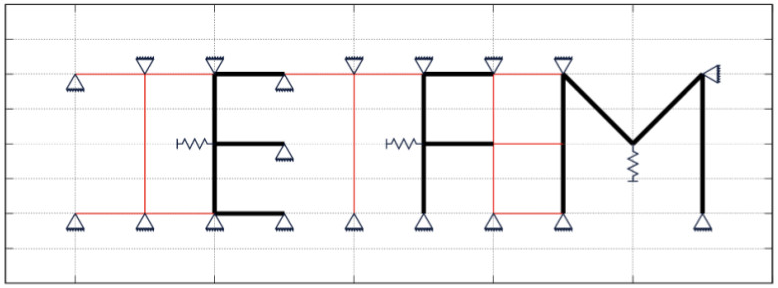
\includegraphics[width=.95\textwidth]{../../../../../../sources/Figs/logo_ietfem}      
\end{center}       
\vspace{0.5cm}       

% hace índice        
%\tableofcontents     

================== Linear Stress IETFEM v2.11 ===========================\\\\


Solve time: $256.464$ seconds \\

Inputfile: \verb|../../input/3D/Truss_3D_sd/torre.txt|  ... \\

Problem type: Truss 3D small deformations and displacements\\ 

Force magnitude: N \\

Length magnitude: m \\

Number of elements: 25 \\

\newpage       

Linear Elasticity:\\

\begin{center}                                   
\begin{longtable}{|R{1.5cm}|R{2.6cm}|}                      
\toprule[0.8mm]                                  
\multicolumn{2}{|c|}{Linear stress} \\      
\midrule[0.5mm]                                  
Element   &   Stress (N/m$^\text{2}$)                  \\         
\midrule[0.5mm]                                  
\endfirsthead                                    
\toprule[0.8mm]                                  
\multicolumn{2}{|c|}{Linear stress} \\      
\midrule[0.5mm]                                  
Element   &   Stress (N/m$^\text{2}$)                  \\         
\midrule[0.5mm]                                  
\endhead                                         
\hline                                           
\multicolumn{2}{r}{Next page...}                 
\endfoot                                         
\endlastfoot                                     
    1 &         1.79 $\times 10^{           6}$ \\
    2 &        -1.77 $\times 10^{           7}$ \\
    3 &        -1.56 $\times 10^{           7}$ \\
    4 &         1.05 $\times 10^{           7}$ \\
    5 &         1.25 $\times 10^{           7}$ \\
    6 &        -2.70 $\times 10^{           7}$ \\
    7 &         1.68 $\times 10^{           7}$ \\
    8 &        -2.53 $\times 10^{           7}$ \\
    9 &         1.84 $\times 10^{           7}$ \\
   10 &         4.41 $\times 10^{           5}$ \\
   11 &         1.39 $\times 10^{           6}$ \\
   12 &         3.38 $\times 10^{           6}$ \\
   13 &        -3.69 $\times 10^{           6}$ \\
   14 &        -8.65 $\times 10^{           6}$ \\
   15 &         5.51 $\times 10^{           6}$ \\
   16 &        -1.02 $\times 10^{           7}$ \\
   17 &         3.94 $\times 10^{           6}$ \\
   18 &        -1.60 $\times 10^{           7}$ \\
   19 &        -1.63 $\times 10^{           7}$ \\
   20 &         1.12 $\times 10^{           7}$ \\
   21 &         1.08 $\times 10^{           7}$ \\
 {\color{OliveGreen}  22} & {\color{OliveGreen}        2.34 $\times 10^{           7}$} \\
   23 &        -2.96 $\times 10^{           7}$ \\
 {\color{red}  24} & {\color{red}       -3.28 $\times 10^{           7}$}\\
   25 &         2.01 $\times 10^{           7}$ \\
\bottomrule[0.8mm]                               
\caption{Linear Stress}             
\end{longtable}                                  
\end{center}                                     

\end{document}  
